\documentclass[tikz,border=5pt]{standalone}
\usepackage{fontspec}
\setmainfont{Times New Roman}
\usepackage{unicode-math}
\setmathfont{Cambria Math}
\usetikzlibrary{shapes.geometric,positioning,fit,backgrounds,arrows.meta,calc}

\begin{document}
\begin{tikzpicture}[
  ent/.style={rectangle, draw, rounded corners, align=center, minimum height=0.85cm, font=\small},
  app/.style={rectangle, draw, rounded corners, align=center, minimum height=0.85cm, font=\small},
  arrow/.style={-{Stealth[length=2.5mm]}, thick},
  label/.style={font=\scriptsize\itshape},
  role/.style={font=\scriptsize\bfseries, fill=white, fill opacity=0.85, text opacity=1},
]

% ===== Application A (Velocity) =====
\begin{scope}[shift={(0,0)}]
  \node[ent, fill=blue!8] (a_q) at (0, 1.1) {Position};
  \node[ent, fill=orange!8] (a_o) at (2.6, 1.1) {Derivative};
  \node[ent, fill=blue!8] (a_r) at (5.2, 1.1) {Time};
  \node[app, fill=green!8] (a_app) at (2.6, -0.5) {Velocity};
  \draw[arrow] (a_q) -- (a_o);
  \draw[arrow] (a_o) -- (a_r);
  \draw[arrow, gray!60] (a_app.north) -- (a_o.south);
  \node[label, below=0.02cm of a_app] {A: cơ học};
\end{scope}

% ===== Application B (Electric current) =====
\begin{scope}[shift={(0,-2.6)}]
  \node[ent, fill=blue!8] (b_q) at (0, 1.1) {Charge};
  \node[ent, fill=orange!8] (b_o) at (2.6, 1.1) {Derivative};
  \node[ent, fill=blue!8] (b_r) at (5.2, 1.1) {Time};
  \node[app, fill=green!8] (b_app) at (2.6, -0.5) {Current};
  \draw[arrow] (b_q) -- (b_o);
  \draw[arrow] (b_o) -- (b_r);
  \draw[arrow, gray!60] (b_app.north) -- (b_o.south);
  \node[label, below=0.02cm of b_app] {B: điện tử};
\end{scope}

% ===== Application C (Population growth) =====
\begin{scope}[shift={(0,-5.2)}]
  \node[ent, fill=blue!8] (c_q) at (0, 1.1) {Population};
  \node[ent, fill=orange!8] (c_o) at (2.6, 1.1) {Derivative};
  \node[ent, fill=blue!8] (c_r) at (5.2, 1.1) {Time};
  \node[app, fill=green!8] (c_app) at (2.6, -0.5) {GrowthRate};
  \draw[arrow] (c_q) -- (c_o);
  \draw[arrow] (c_o) -- (c_r);
  \draw[arrow, gray!60] (c_app.north) -- (c_o.south);
  \node[label, below=0.02cm of c_app] {C: kinh tế học};
\end{scope}

% ===== Shared invariant structure (abstract) =====
\node[draw, thick, rounded corners, fill=yellow!12, align=center, minimum height=2.2cm, font=\small, text width=4.2cm]
  (inv) at (9.2, -1.3) {%
    \textbf{Cấu trúc bất biến (đề xuất)}\\[4pt]
    Quantity $\xrightarrow{\text{Derivative}}$ Result\\[2pt]
    withRespectTo: Time\\[2pt]
    {\scriptsize\itshape tên miền (Position, Charge,\\ Population) là ngẫu nhiên}
  };

\draw[arrow, dashed, thick] (a_r.east) -- node[label, above, pos=0.5] {trừu tượng hóa} (inv.west);
\draw[arrow, dashed, thick] (b_r.east) -- (inv.west);
\draw[arrow, dashed, thick] (c_r.east) -- (inv.west);

% ===== Hypothesis note =====
\node[label, align=center, text width=5.6cm, below=0.3cm of inv.south]
  {CandidateMechanismHypothesis:\\ "có lẽ cả ba cùng một cơ chế trừu tượng"\\ (ứng viên, chưa được chấp nhận)};

\end{tikzpicture}
\end{document}